\section{Test Generator Plugin}
We have chosen to only focus on Flutter development since it allows us to narrow the technical challenges into a known domain for the members of the group.
We envision a plugin for Flutter that can be installed and will run as part of the test suite in the Flutter application.
Since the Flutter framework has a pre-configured test framework, we envision our plugin to generate code that is compatible with the built-in test environment of Flutter.
Thereby leaving little to no setup required.

We envision our plugin to be configured to connect to the task and screen definitions from the application using a shared backend API.
Our plugin will then be able to parse the data structure used by the Mobile Customer Application to automatically generate executable tests.

We can already see some big issues with this approach such as:
The developer may have no or an unstable internet connection.
Implementation details that are not part of the knowledge domain of the Mobile Customer Application, such as data management layer or authentication strategies, are none standard for Flutter and does thus require the user to specify these details.

\figur{1}{images/idea-overview.png}{A rough sketch of the system}{fig:ideaoverview}

Therefore we envision a compromise from our initial idea. 
We will still build a plugin, but instead of building a Flutter only plugin, we will build a more general package that can be used either in a Flutter project or in a stand-alone project.
Such a general package would allow the development team to have full control over how their tooling pipeline is constructed.

For some development teams, it would be fine to have our solution coupled directly into the implementation code base, as shown on~\autoref{package_in_futter}, for other teams, it would be seen as a risk to rely so heavily on third-party tooling, and they can instead create a simple program that uses our package and thereby decouple their implementation codebase from our package, as shown on~\autoref{package_outside_flutter}. 

The package should then have the ability to connect to the backend and generate the test suite - the output would then be what we will call the test artefacts.

\begin{figure}[H]
    \centering
    \begin{minipage}{0.45\textwidth}
        \centering
        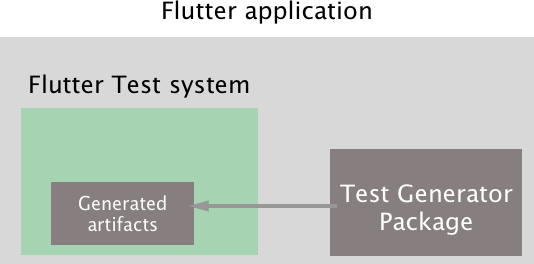
\includegraphics[width=0.9\textwidth]{images/Embedded-in-flutter.png}
        \caption{Diagram of the package inside a Flutter project.}
        \label{package_in_futter}
    \end{minipage}\hfill
    \begin{minipage}{0.45\textwidth}
        \centering
        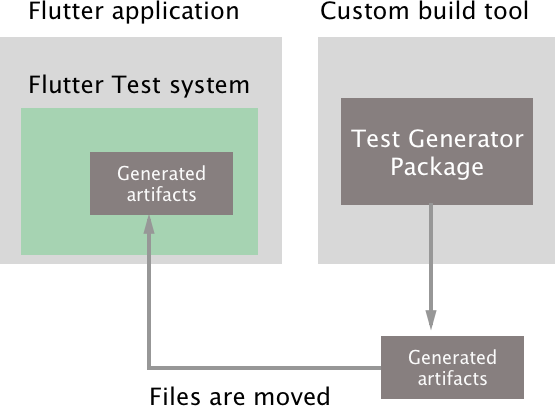
\includegraphics[width=0.9\textwidth]{images/Decoupled-from-flutter.png}
        \caption{Diagram of the package decoupled from Flutter project.}
        \label{package_outside_flutter}
    \end{minipage}
\end{figure}

The test artefacts are simply the generated target code exported to files and stored on the disc. 
If the developer team has chosen to use our package in their Flutter implementation codebase the package could be configured to override the old artefacts and repopulate with the new ones.
If the developer team has chosen to decouple our package, it is up to them to decide how they would like the process to be.
They could choose to make it fully manually, so the developer has to copy and paste the artefacts into the implementation, or they could automate it into their tooling.

This means that if the developer does not have internet access and thereby cannot get the newest tests, they can simply run the old test artefacts and generate the new test artefacts whenever regaining access to the internet.
Another benefit of this is the execution time, not having to make an HTTP-roundtrip every time the developer runs the tests, will make the whole test suite run faster.

The next compromise is about boundaries of the test artefacts we generate, these artefacts are only concerned with acceptance tests, meaning the most outer layer of the system under test. 
This also means that our test artefacts should not be tightly coupled to implementation details, as we trust in the craftsmanship of the developers and assume that they have tested the implementation details themselves.
We take the stand that the actual implementation is a black box for our artefacts, and to do so we have to segregate our test artefacts from the system under test.
We believe this can be done by having the test generator create an interface that should be used to run the test artefacts.
This interface should then be implemented by the developers, which will allow the test artefacts to request the interface for a "login page".

Another use case we envision for the segregation interface is for functionalities such as authentication, rather our test artefacts know how to authenticate users and check a given user authentication, we can simply ask the interface to authenticate a given user or to report back on the authentication status of said user.
Since the implementation of the interface is done by the developers they also can swap implementations as they please, which can be beneficial e.g. when having to use mocks or spies instead of a real implementation.

Another benefit of the segregation interface is that we can have data structures known by the users of the Mobile Customer Application, but allow the developers to use whatever data structures they see fit.
Imagine the interface specifying a factory-method for a user, when implementing the developer can use the actual system data structure or structures for representing a user and simply inject it into the one specified in the Mobile Customer Application.
Thereby allowing total freedom to the developers while still having the ability to create tests that depend on specific data structures.

On~\autoref{fig:ideaoverview} there is a rough sketch of how we envision the entire eco-system to work.
